\myparagraph{Purpose}
Everytime a special user wants to access to the data of a group of people it has to specify at least one of the required characteristics of it:
\begin{itemize}
  \item It can choose among the age ranges of the members of the targeted group proposed by the system;
  \item It can specify the Italian city of birth of the members of the targeted group;
  \item It can specify the Italian city of residence of the members of the targeted group;
  \item It can specify the Italian province of residence of the members of the targeted group;
  \item It can specify the Italian province of birth of the members of the targeted group;
  \item It can specify the Italian region of residence of the members of the targeted group;
  \item It can specify the Italian region of birth of the members of the targeted group;
  \item It can specify the state of birth of the members of the targeted group;
  \item It can specify the state of residence of the members of the targeted group;
  \item It can specify the current occupation (students, employeds, unemployeds) of the members of the targeted group.
\end{itemize}
After this the system will check if the targetd group is composed of more than 1000 people, if it is, the special user will receieve the payment form with the amount it has to pay to download the required data. Once it pays the amount due it can download the required data.

\myparagraph{Scenario 1}
PharmaAnalisi SPA wants to acquire data of a group of students living in Lombardia in order to do an analysis about the kind of life they conduct. It opens the browser and search for \textit{Data4Help} web site, then it logs in and goes in "\textit{Data Search}" area. It specifies that the age range of the members of the targeted group must be from 18 to 24 years old, that they should live in a city in Lombardia and that they should be students. Then it clicks on the "\textit{Submit}" button and the system accepts its request, PharmaAnalisi SPA receives the payment form with the amount it has to pay, it pays the amount due and it downloads the required data.

\myparagraph{Scenario 2}
The municipality of Sondrio wants to analyze the quality of life of the people that were born in Monza and that moved to Sondrio.  It opens the browser and search for \textit{Data4Help} web site, then it logs in and goes in "\textit{Data Search}" area. It specifies that the city of birth of the members of the targeted group must be Monza and that their city of residence must be Sondrio. Then it clicks on the "\textit{Submit}" button but unfortunately the system tells that the required data aren't accessible because the targeted group of people is composed of less than 1000 people and so the process ends.

\myparagraph{Use Case}
The \textit{Group Data Requirement} use case is analyzed in Table \ref{table:groupDataRequirement}.

\myparagraph{Activity Diagram}
The \textit{Group Data Requirement} activity diagram is shown in Figure \ref{img:groupDataRequirementActivityDiagram}.

\myparagraph{Mockup}
The \textit{Group Data Requirement} mockup is shown in Figure \ref{img:individualDataRequirementMockup}.

\myparagraph{Functional requirements}
\begin{enumerate}
  \item The system must not give data of groups of people composed of less than 1000 people;
  \item The system must not let the special user download the required data untill it hasn't paid the amount due;
  \item The system must let the \textbf{Special user} leave the data requirement process at anytime.
\end{enumerate}

\begin{center}
\begin{table}[H]
\begin{tabular}{ | l | p{0.75\linewidth} | }
  \hline
    Actor & \textbf{Special user}\\ \hline
    Goal & \textbf{[G.5]} \\ \hline
    Input Condition & A \textbf{Special user} wants to acquire data of a group of people \\ \hline
    Event Flow & \begin{minipage}[t]{0.7\textwidth}
      \begin{enumerate}
        \item The \textbf{Special user} opens the main page of \textit{Data4Help} web site;
        \item The \textbf{Special user} logs in;
        \item The \textbf{Special user} goes in "\textit{Data Search}" area;
        \item The \textbf{Special user} specifies the characteristics of the targeted group;
        \item The \textbf{Special user} clicks on "\textit{Submit} button;
        \item If the targeted group is composed of more than 1000 people the \textbf{Special user} receieves the payment form with the amount it has to pay to download the required data;
        \item The \textbf{Special user} pays the amount due;
        \item The \textbf{Special user} downloads the required data.
      \end{enumerate}
    \smallskip
  \end{minipage} \\ \hline
  Output Condition & The \textbf{Special user} receives the required data \\ \hline
  Exceptions & \begin{minipage}[t]{0.7\textwidth}
    \begin{itemize}
      \smallskip
      \item If the targeted group is composed of less than 1000 people the \textbf{Special user} is informed and the process is aborted;
      \item If functional requirement 2 is not satisfied the process goes back to step 7;
      \item If the \textbf{Special user} decides to leave the data requirement process this one is aborted.
    \end{itemize}
    \smallskip
  \end{minipage}  \\ \hline
\end{tabular}
\caption{\textit{Group Data Requirement} use case}
\label{table:groupDataRequirement}
\end{table}
\end{center}

\begin{figure}[H]
\begin{center}
  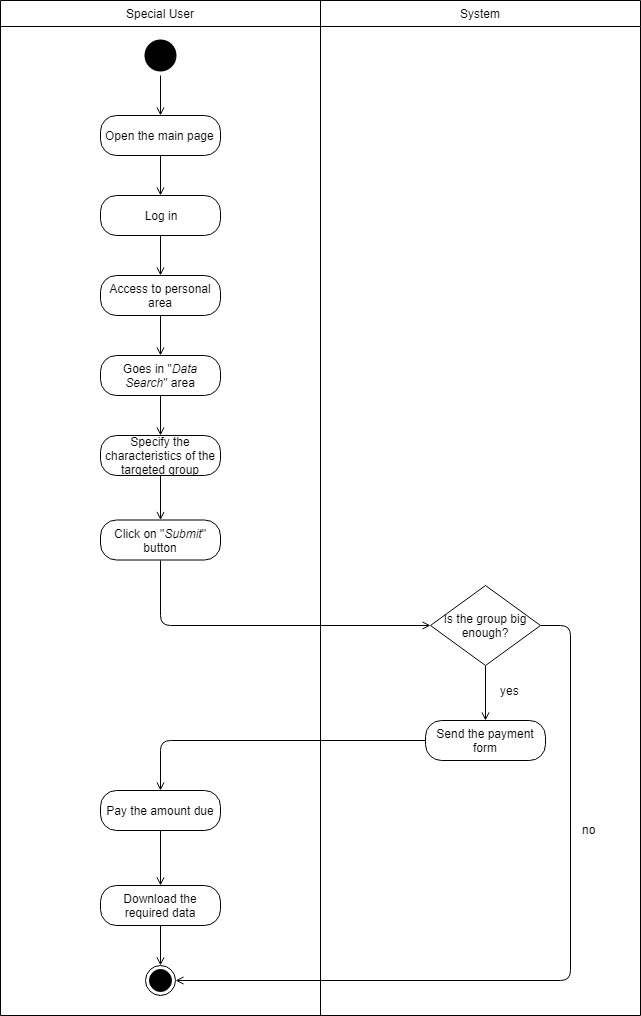
\includegraphics[height=0.6\paperheight]{img/activity/GroupDataRequirement.png}
  \hspace{0.05\linewidth}
  \centering
  \caption{\textit{Group Data Requirement} activity diagram}
  \label{img:groupDataRequirementActivityDiagram}
\end{center}
\end{figure}
